\resizebox{\columnwidth}{!}{%
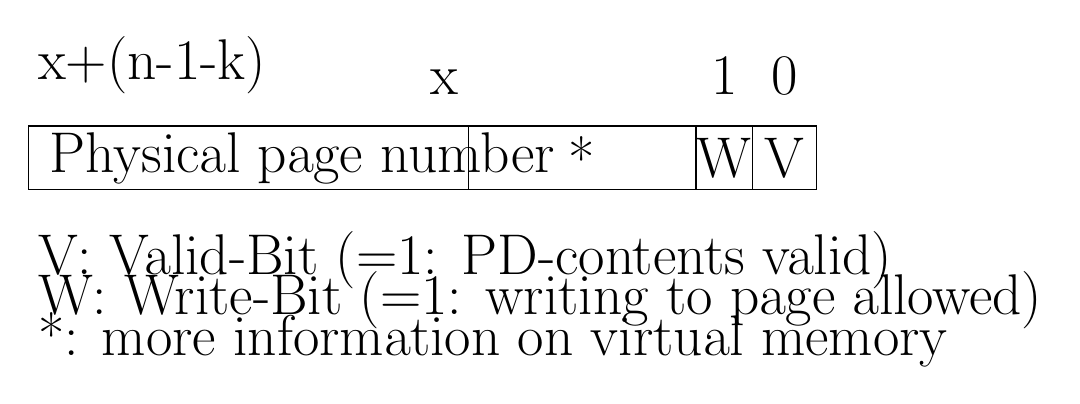
\begin{tikzpicture}[font=\huge]

% ---------- column boundaries (measured from source) ----------
% left=0, div1=8.586 (end of "Physische Page-Nummer"), div2=11.48 (end of "*"),
% div3=12.20 (end of "W"), right=13.01 (end of "V")
% box: top y=0, bottom y=-0.81

% ---------- top bit-position labels ----------
\node[anchor=south west] at (0,0.28) {x+(n-1-k)};
\node[anchor=south east] at (5.586,0.28) {x};
\node[anchor=south] at (8.84,0.28) {1};
\node[anchor=south] at (9.605,0.28) {0};

% ---------- the box ----------
\draw (0,0) rectangle (10.01,-0.81);
\draw (5.586,0) -- (5.586,-0.81);
\draw (8.48,0) -- (8.48,-0.81);
\draw (9.20,0) -- (9.20,-0.81);

% ---------- box field text ----------
\node[anchor=west] at (0.15,-0.405) {Physical page number};
\node at (7.03,-0.405) {*};
\node at (8.84,-0.405) {W};
\node at (9.605,-0.405) {V};

% ---------- legend ----------
\node[anchor=north west] at (0,-1.215) {V: Valid-Bit (=1: PD-contents valid)};
\node[anchor=north west] at (0,-1.728) {W: Write-Bit (=1: writing to page allowed)};
\node[anchor=north west] at (0,-2.241) {*: more information on virtual memory};

\end{tikzpicture}
}